\clearpage
\section*{\currfilename}

\begin{figure}[H]
  \fontsize{10pt}{10pt}\selectfont
  \begin{center}
    \resizebox{3.0in}{1.0in}{
      \begin{tikzpicture}[auto, scale=1.0, every node/.style={transform shape}, node distance=1.0cm, >=latex']
        \node[squareblock, minimum height=1cm, minimum width=2cm] (block1){Baseline};
        \node[squareblock, below of=block1, node distance=1.5cm, minimum height=1cm, minimum width=2cm] (block2){Adaptive};

        \matrix[ampersand replacement=\&, row sep=0.5cm, left of=block1,node distance=1cm] (block1in) {
          \node [coordinate] (b1inA) {}; \\
          \node [coordinate] (b1inB) {}; \\
        };

        \matrix[ampersand replacement=\&, row sep=0.5cm, left of=block2,node distance=1cm] (block2in) {
          \node [coordinate] (b2inA) {}; \\
          \node [coordinate] (b2inB) {}; \\
        };

        \node[whitesum,right of=block1, node distance=2.0cm] (sum1) {};
        \node [right of=sum1,draw=black, node distance=3.5cm, label=below:{\shortstack[c]{Equations of\\Motion}}, minimum width=2cm, inner sep= 0mm] (block3) {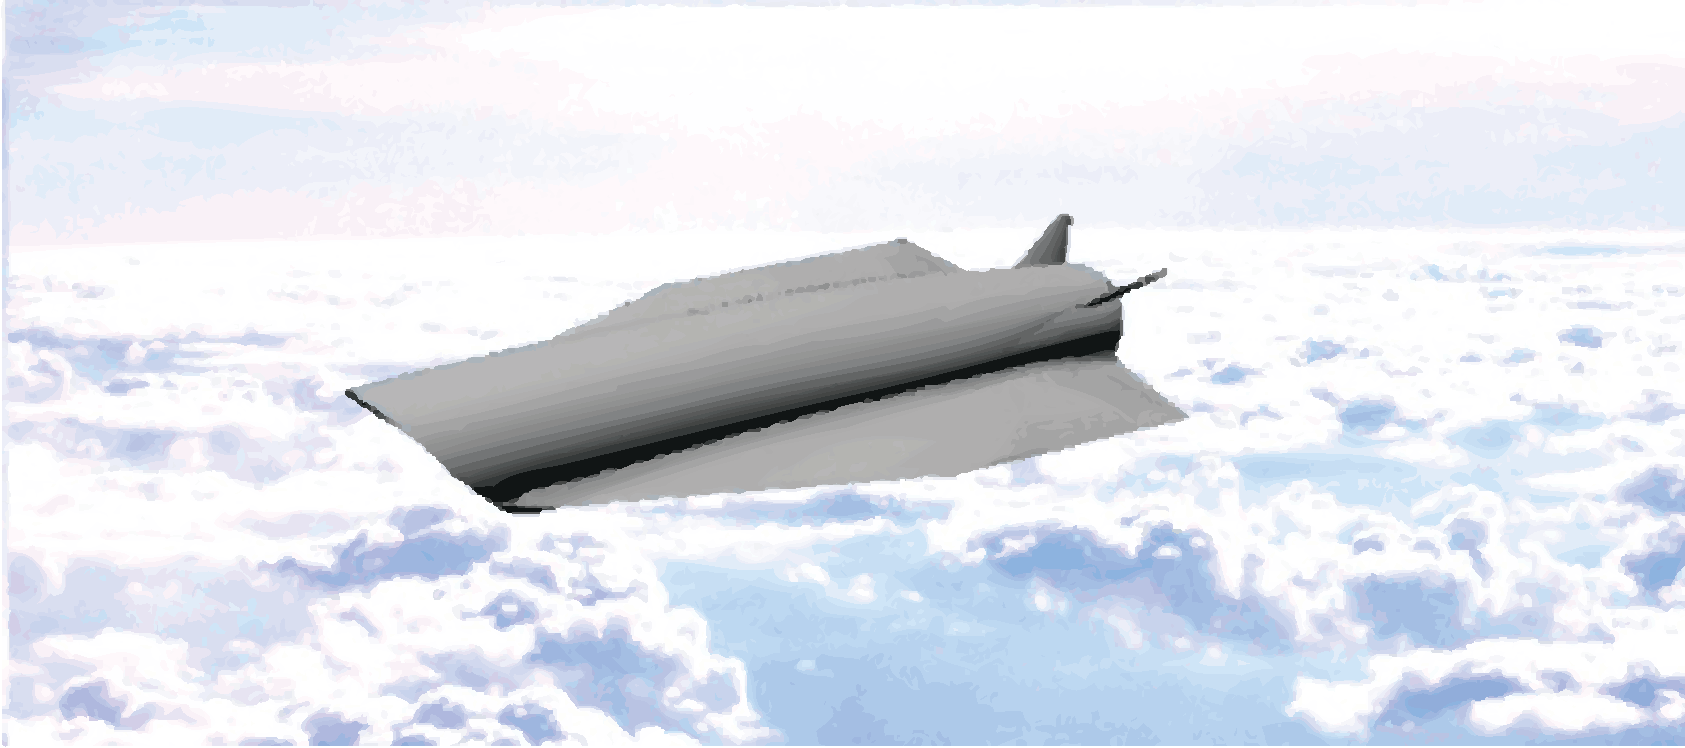
\includegraphics[width=4cm]{../fig/ghvclouds.pdf}};
        \node[squareblock, minimum height=1cm, minimum width=2cm, above of=block3,node distance=1.75cm] (block4) {\shortstack[c]{Reference\\Model}};
        \node[whitesum,right of=block3, node distance=3.5cm] (sum2) {};
        \node[input,below of=block2, node distance=1.5cm] (input2) {};
        \node[output,right of=sum2, node distance=1.5cm] (output1) {};

        % Gray shaded box
        \begin{pgfonlayer}{background}
          \path (block1 |- block1)+(-2.5,0.7) node (c) {};
          \path (block2 -| block2)+(2.5,-0.7) node (d) {};
          \path[fill=gray!20, draw, dashed] (c) rectangle (d);
        \end{pgfonlayer}

        % Draw
        \draw [->]  (b1inA) + (-2.5cm,0cm) -> node [pos=0.0]{$z_{\text{cmd}}$}  (b1inA);
        \draw [->]  (b1inA) + (-2.0cm,0cm) |- node [pos=0.15]{}  (block4);
        \draw [->]  (b1inB) + (-0.5cm,0cm) -> (b1inB);
        \draw [->]  (b2inA) + (-1cm,0cm) -> (b2inA);
        \draw [->]  (b2inB) + (-2.0cm,0cm) -> (b2inB);
        \draw [-]  (b2inB) + (-2.0cm,0cm) |- (input2);
        \draw[->](block3) --  node[name=yi,pos=0.3]{$x_{p}$} node[pos=0.9]{$+$} (sum2);
        \draw[-](yi) |- (input2);
        \node [coordinate, left of=b1inB, node distance=0.5cm] (b1inBleft) {};
        \node [coordinate, left of=b2inA, node distance=1.0cm] (b2inAleft) {};
        \draw [-]  (b1inBleft) + (0.0cm,-1.5cm) -- (b1inBleft);
        \draw [-]  (b2inAleft) + (0.0cm,1.5cm) -- (b2inAleft);
        \draw[->](block1) -- node[pos=0.7]{$+$} (sum1);
        \draw[->](block2) -| node[pos=0.9]{$+$} (sum1);
        \draw[->](sum1) -- node[pos=0.6]{$u$} (block3);
        \draw[->](block4) -| node[pos=0.1]{$x_{m}^{o}$} node[pos=0.95]{$-$} (sum2);
        \draw[->](sum2) -- node[pos=0.4]{$e^{o}$} (output1);
      \end{tikzpicture}
    }
    \caption{\fontsize{7pt}{7pt}\selectfont \textbf{Classical open loop reference model adaptive control architecture}}
  \end{center}
\end{figure}
